\chapter{Alternative Mitigation Strategies}
\epigraph{There's no silver bullet solution with cybersecurity; a layered defense is the only viable defense.}{\textit{James Scott}}

Nintendo's response to the Fusee Gelee exploit, involving both hardware revisions and software updates, has been largely effective in mitigating the immediate vulnerability. The introduction of the Mariko chip with a corrected Boot ROM and the release of new hardware models have addressed the specific buffer overflow issue exploited by Fusee Gelee. However, these measures have limitations, particularly in terms of financial accessibility for users and the residual vulnerability of older Switch models. Additionally, even the new consoles, while more secure, remain susceptible to hacking through more complex methods requiring advanced tools and techniques

\section{Proposed Solutions}
To further enhance the security of hardware like the Nintendo Switch, additional strategies beyond those implemented by Nintendo could be considered. These strategies aim to provide more comprehensive protection but come with their own set of drawbacks.

\subsection{Hardware-Level Solutions}
\subsubsection{Secure Enclave Integration}

One effective method for enhancing hardware security is the integration of secure enclaves. Secure enclaves are isolated execution environments within the processor that perform sensitive operations, such as cryptographic key storage and execution of critical code, in a protected manner.\cite{IntroductionHardwareSecurity}

\begin{figure}[H]
    \centering
    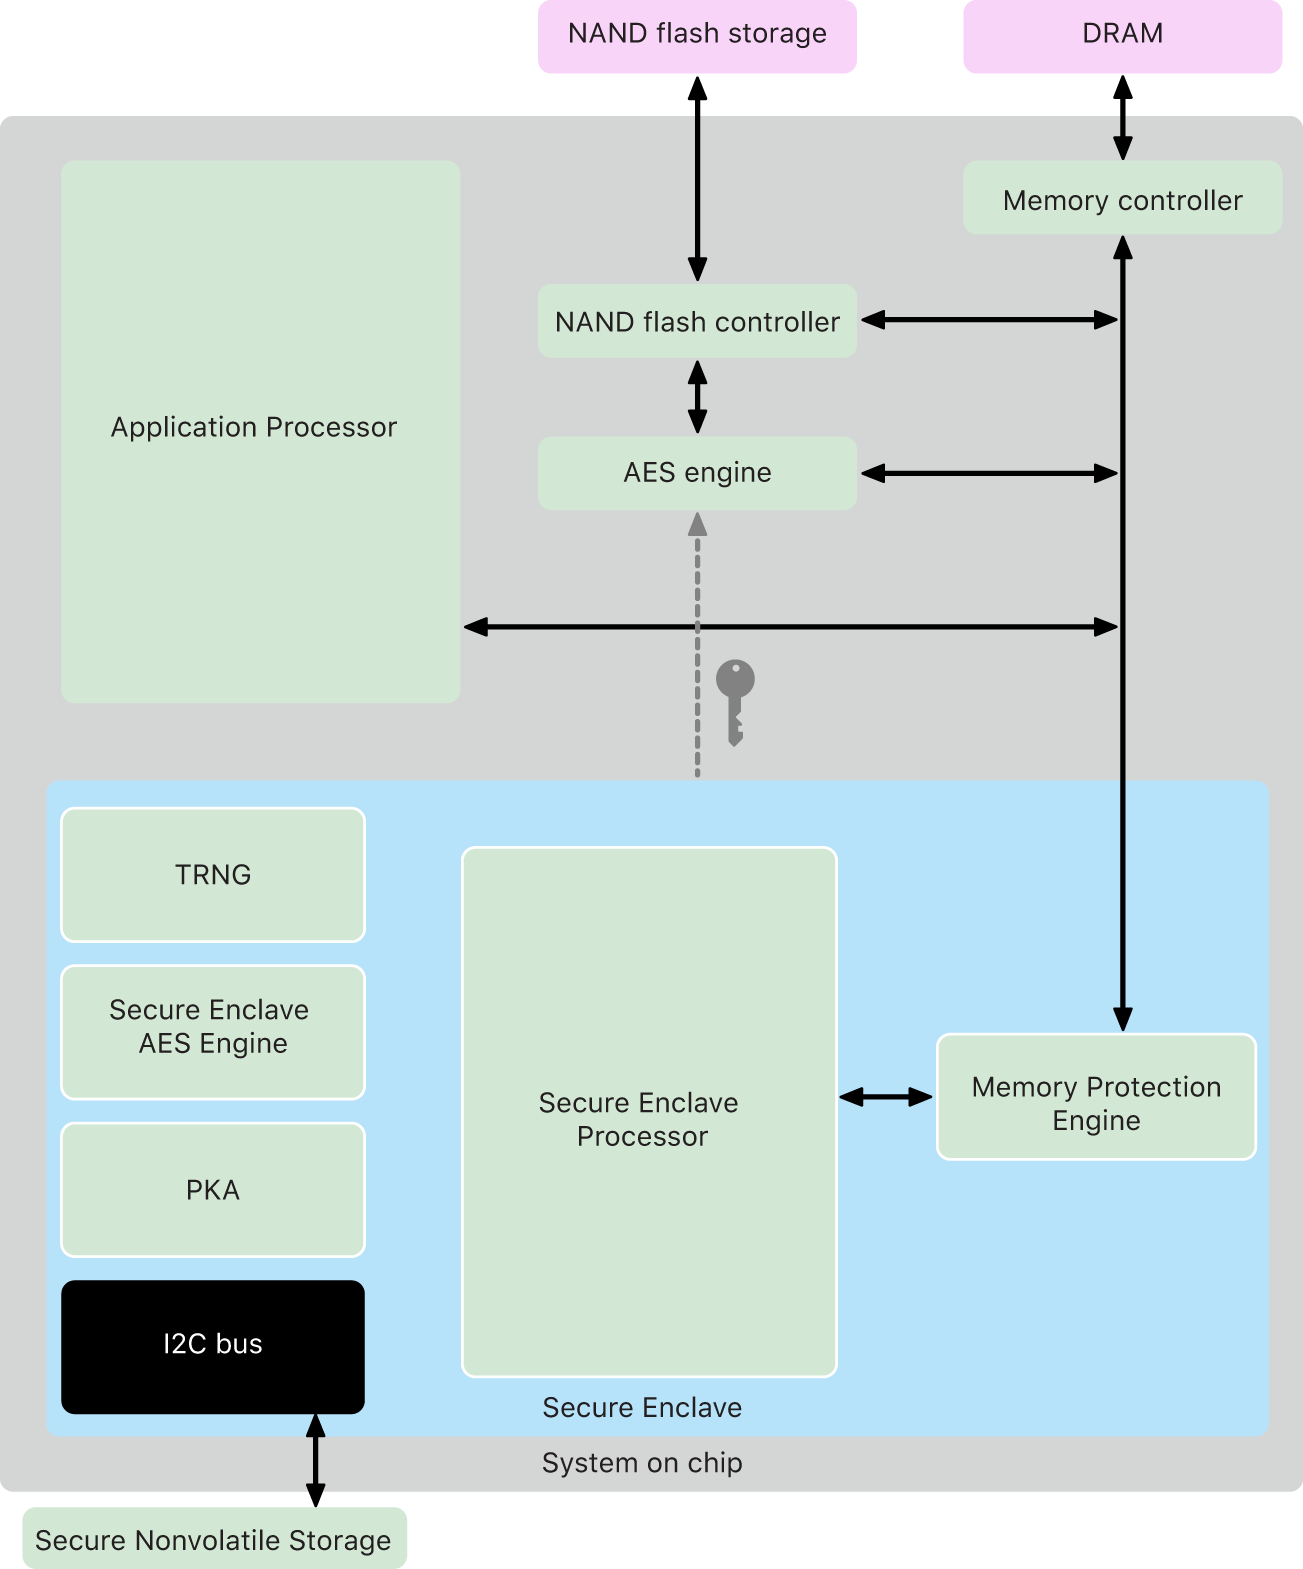
\includegraphics[width=.8\linewidth]{images/enclave.png}
    \caption{Secure Enclave Architecture from\cite{SecureEnclave}}
    \label{fig:secure_enclave}
\end{figure}

\subsubsection{Advantages}

\begin{itemize}
    \item \textbf{Enhanced Security}: Secure enclaves provide robust protection against a wide range of attacks, including those targeting the Boot ROM and other critical components.
    \item \textbf{Root of Trust}: They establish a hardware-based root of trust, ensuring that even if other parts of the hardware are compromised, sensitive operations remain secure.
\end{itemize}
\subsubsection{Drawbacks}

\begin{itemize}
    \item \textbf{Increased Cost}: Integrating secure enclaves into the hardware design significantly increases manufacturing costs.
    \item \textbf{Complexity}: It adds complexity to the hardware design and development process, potentially leading to longer development cycles and higher production costs
\end{itemize}
\subsubsection{Redundant Security Mechanisms}
Incorporating redundant security mechanisms\cite{RedundancyEngineering2023} can provide multiple layers of defense against hardware vulnerabilities. For example, dual verification processes during the boot sequence, where both the Boot ROM and a secondary chip verify each other's integrity, can enhance security.

\subsubsection{Advantages}

\textbf{Increased Reliability}: Multiple layers of verification reduce the likelihood of successful exploitation.
\textbf{Fault Tolerance}: Redundant systems provide a fallback in case one security measure is compromised.
\subsubsection{Drawbacks}

\begin{itemize}
    \item \textbf{Design Complexity}: Implementing redundant mechanisms increases the complexity of the hardware design.
    \item \textbf{Cost and Power Consumption}: Additional components and verification processes can increase both the cost and power consumption of the device.
\end{itemize}


\begin{figure}[H]
    \centering
    \begin{tikzpicture}[
        box/.style={rectangle, draw, text width=8em, align=center, rounded corners},
        arrow/.style={-Stealth, thick},
        level distance=2cm
      ]
      
      % Nodes
      \node[box] (bootrom) {Boot ROM Initiates Boot};
      \node[box, below=of bootrom] (verify1) {Verifies Secondary Chip Integrity};
      \node[box, below=of verify1] (secondary) {Secondary Chip Firmware};
      \node[box, right=of verify1, xshift=2cm] (verify2) {Verifies Boot ROM Integrity};
      
      % Paths
      \draw[arrow] (bootrom) -- (verify1);
      \draw[arrow] (verify1) -- (secondary);
      \draw[arrow] (secondary) -- ++(1.5cm, 0) |- (verify2);
      \draw[arrow] (verify2) -- ++(-1.5cm, 0) |- (verify1);
    \end{tikzpicture}
    \caption{Redundant Security Mechanisms in Boot Sequence}
    \label{fig:redundant_security}
\end{figure}

In conclusion, while Nintendo's response to the Fusee Gelee exploit has been effective to a large extent, further enhancements could be made by adopting advanced hardware. These measures, however, come with significant drawbacks, highlighting the inherent challenges in achieving complete security in consumer hardware devices. Future hardware designs must balance these trade-offs to ensure robust security while maintaining cost-effectiveness and performance.